\documentclass[a4paper,12pt]{article} 
\usepackage{geometry}
\usepackage{wrapfig}
\geometry{
	a4paper,
	total={170mm,257mm},
	left=10mm,
	right=10mm,
	top=20mm,
}
\usepackage{titlesec}
\titlelabel{\thetitle.\quad} %точка в section

%%% Работа с русским языком
\usepackage{cmap}                           % поиск в PDF
\usepackage{mathtext} 			 	       % русские буквы в формулах
\usepackage[T2A]{fontenc}               % кодировка
\usepackage[utf8]{inputenc}              % кодировка исходного текста
\usepackage[english,russian]{babel}  % локализация и переносы

%Математика
\usepackage{amsmath,amsfonts,amssymb,amsthm,mathtools} % AMS
\usepackage{icomma} % "Умная" запятая

%% Шрифты
\usepackage{euscript}	 % Шрифт Евклид
\usepackage{mathrsfs} % Красивый матшрифт

\usepackage{gensymb}
\usepackage{graphicx}
\usepackage{setspace}
\usepackage{tabularx}
\usepackage{longtable}
\usepackage{icomma}
\usepackage{euscript}
\usepackage{float}
\usepackage{cutwin}
\usepackage{adjustbox}
\usepackage{dashbox}
\usepackage[normalem]{ulem}	
\usepackage[babel=true]{microtype}
\RequirePackage[T1]{fontenc}
\usepackage{amsmath,amsfonts,amssymb,amsthm,mathrsfs,mathtools} 
\usepackage{xcolor}         
\usepackage{enumitem}     
\usepackage{xpatch}       
\usepackage{cancel}                  
\usepackage{upgreek}                 
\usepackage{lipsum}                  
\usepackage[version=4]{mhchem}       
\usepackage{multirow}                
\usepackage{stackengine}             
\usepackage{tikz}         
\usepackage{hyperref}
\hypersetup{colorlinks=true,urlcolor=blue}       
\usetikzlibrary{positioning}         
\usepackage{titletoc}                 
\usepackage{chngcntr}              
\usepackage{fancyhdr}                
\usepackage{makecell}                
\usepackage{indentfirst}             
\usepackage{tocloft}                 
\usepackage{soul}                   
\usepackage[stable]{footmisc}       
\usepackage{subfig}  
\usepackage{comment}                  


\mathtoolsset{showonlyrefs=true}


\theoremstyle{definition}
\newtheorem*{definition}{Определение}
\newtheorem{statement}{Предложение}[section]
\newtheorem{lemma}{Лемма}[section]
\newtheorem{theorem}{Теорема}[section]
\newtheorem*{theoremn}{Теорема}
\newtheorem*{corollary}{Следствие}
\newtheorem*{example}{Пример}
\newtheorem*{note}{Замечание}
\newtheorem*{problem}{Задача}


\counterwithout{footnote}{section}\DeclareRobustCommand{\divby}{%
	\mathrel{\text{\vbox{\baselineskip.65ex\lineskiplimit0pt\hbox{.}\hbox{.}\hbox{.}}}}%
}

\newcommand{\dotpr}[2]{\bra{#1}\ket{#2}}
\let\emptyset\varnothing
\DeclareMathOperator*{\esssup}{ess sup}
\DeclareMathOperator*{\ord}{ord}
\DeclareMathOperator*{\supp}{supp}
\DeclareMathOperator*{\pr}{pr}
\DeclareMathOperator*{\Ker}{Ker}
\DeclareMathOperator*{\Vol}{Vol}
\DeclareMathOperator*{\rg}{rk}
\DeclareMathOperator*{\Ima}{Im}
\DeclareMathOperator*{\Alt}{Alt}
\DeclareMathOperator*{\Sym}{Sym}
\newcommand{\eqdef}{\stackrel{\text{\tiny{def}}}{=}}
\newcommand{\pp}{\partial}
\newcommand{\aA}{\mathcal{A}}
\newcommand{\BB}{\mathcal{B}}
\newcommand{\MM}{\mathbb{M}}
\newcommand{\NN}{\mathbb{N}}
\newcommand{\ZZ}{\mathbb{Z}}
\newcommand{\QQ}{\mathbb{Q}}
\newcommand{\RR}{\mathbb{R}}
\newcommand{\CC}{\mathbb{C}}
\newcommand{\FFF}{\mathbb{F}}
\newcommand{\DD}{\mathcal{D}}
\newcommand{\FF}{\mathcal{F}}
\newcommand{\sS}{\mathcal{S}}
\newcommand*\circled[1]{\tikz[baseline=(char.base)]{
		\node[shape=circle,draw,inner sep=2pt] (char) {#1};}}

%%% Заголовок
\author{Шерхалов Денис Б02-204и \\
		Фаттахов Марат Б02-204кт}
\title{Лабораторная работа 5.1.1 \\
	\textbf{Фотоэффект}}
\date{\today}

\begin{document}
	
{\Large \maketitle}

\textbf{В работе}: исследовать зависимость фототока от величины задерживающего потенциала и частоты падающего излучения, что позволяет вычислить величину постоянной Планка.

\section{Введение}

    Фотоэффект --- явление испускания электронов фотокатодом, облучаемым светом,  Это явление хорошо объясняется фотонной теорией света. Взаимодействие монохроматического света с веществом можно описывать
	как взаимодействие с веществом частиц, называемых фотонами, которые обладают энергией $ \hbar \omega $ и импульсом $ \hbar\omega/c $. При столкновении фотона с электроном фотокатода энергия отона полностью передается электрону, и фотон прекращает свое существование. Энергетический баланс этого взаимодействия для вылетающих электронов
	описывается уравнением
	
	\begin{equation}\label{energy balance}
	\hbar \omega = E_{\text{кин}} + A_{\text{вых}}
	\end{equation}
	
	\begin{wrapfigure}{l}{0.4\linewidth}
		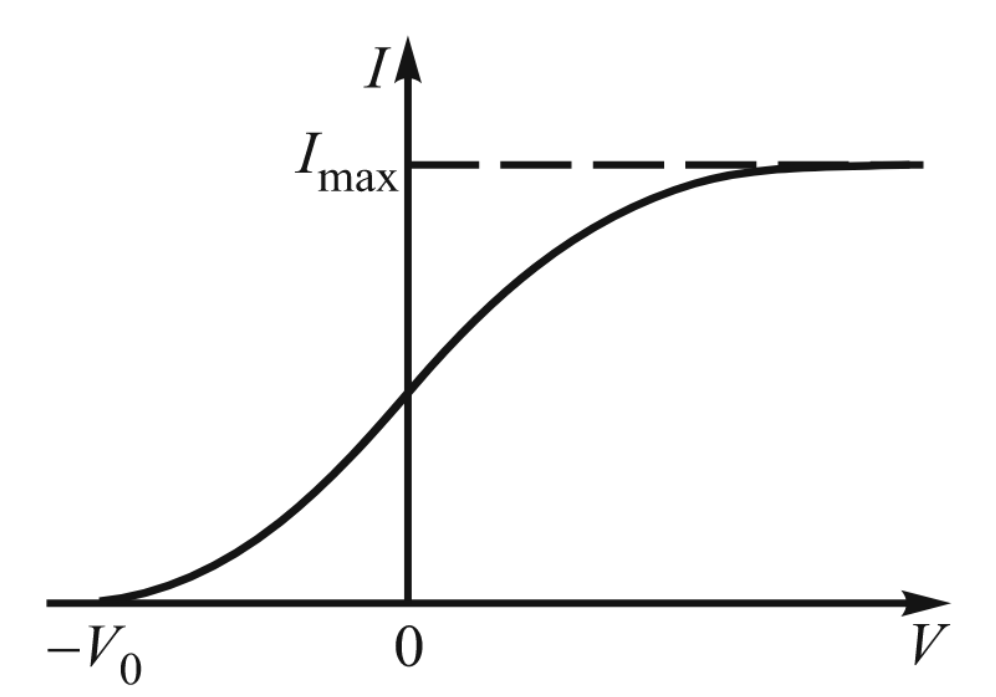
\includegraphics[width=\linewidth]{I_V.png}
		\caption{Зависимость фототока от напряжения на аноде фотоэлемента}
		\label{ris I(V)}
	\end{wrapfigure}
	
	Здесь $E_{\text{кин}}$ ---  максимальная кинетическая энергия электрона после выхода из фотокатода, $A_{\text{вых}}$ --- работа выхода электрона из катода. Реально энергетический спектр вылетевших из фотокатода электронов непрерывен --- он простирается от нуля до $ E_{\text{кин}} $. 
	
	Для измерения энергии вылетевших фотоэлектронов вблизи фотокатода
	обычно располагается второй электрод
	(анод), на который подается задерживающий ($ V < 0 $) или ускоряющий ($ V >
	0 $) потенциал. При достаточно больших
	ускоряющих напряжениях фототок достигает насыщения (рис. \ref{ris I(V)}): все испущенные электроны попадают на анод.
	
	При задерживающих потенциалах на анод попадают лишь электроны,
	обладающие достаточно большой кинетической энергией, в то время
	как медленно движущиеся электроны заворачиваются полем и возвращаются на катод. При некотором значении $ V = -V_0 $ (потенциал запирания) даже наиболее быстрые фотоэлектроны не могут достичь
	анода.
	Максимальная кинетическая энергия $E_{\text{кин}}$ электронов связана с
	запирающим потенциалом $ V_0 $ очевидным соотношением $ E_{\text{кин}} = eV_0 $. Тогда \eqref{energy balance} примет вид, называемый уравнением Эйнштейна:
	
	\begin{equation}\label{Einsteain}
	eV_0 = \hbar\omega - A_{\text{вых}}
	\end{equation}
	
	Чтобы определить величину запирающего
	напряжения, нам надо правильно экстраполировать получаемую токовую зависимость к нулю, т. е. определить, какова функциональная
	зависимость $ I(V) $. Расчет для простейшей геометрии --- плоский катод, освещаемый светом, и параллельный ему анод --- приводит к зависимости
	
	\begin{equation}\label{sqrt I = V}
	\sqrt{I} \propto V_0 - V
	\end{equation}
	
	т. е. корень квадратный из фототока линейно
	зависит от запирающего напряжения. Эта зависимость хорошо описывает экспериментальные данные.
	
	В работе изучается зависимость фототока из фотоэлемента от величины задерживающего потенциала $ V $ для различных частот света $ \omega $, лежащих в видимой области спектра. С целью экспериментальной
	проверки уравнения Эйнштейна определяются потенциалы запирания
	$ V_0 $ при разных частотах света и строится зависимость $ V_0(\omega) $, которая, как это следует из \eqref{Einsteain}, должна иметь вид
	
	\begin{equation}\label{V(w)}
	V_0 (\omega) = \dfrac{\hbar\omega - A_{\text{вых}}}{e}
	\end{equation}
	
		\begin{wrapfigure}{r}{0.4\linewidth}
		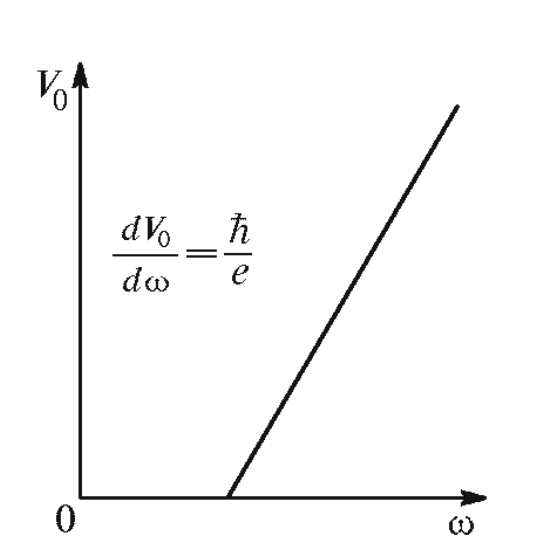
\includegraphics[width=\linewidth]{V_w.png}
		\caption{Зависимость запирающего потенциала
			от частоты света}
		\label{ris V(w)}
	\end{wrapfigure}
	
	Потенциал запирания $ V_0 $ для любого катода линейно зависит от
	частоты света $ \omega $. По наклону прямой на графике $ V_0(\omega) $ (рис. \ref{ris V(w)}) можно определить постоянную Планка:
	
	\begin{equation}\label{dV/dw}
	\dfrac{dV_0}{d\omega} = \dfrac{\hbar}{e}
	\end{equation}
	
	Как показывает формула \eqref{dV/dw}, угол наклона прямой $ V_0(\omega) $ не зависит от рода вещества, из которого изготовлен фотокатод. От рода вещества, однако, зависит величина фототока, работа выхода $ W $ и форма кривой $ I(V) $ (рис. \ref{ris I(V)}). Все это определяет выбор пригодных для
	опыта катодов.

    \section{Выполнение}
	
	Сначала выполним градуировку монохроматора. Проведем серию измерений для линий спектра неона, снимая зависимость длины волны света от параметра $ \theta $ 
	барабана монохроматора. Результаты занесем в Таблицу 1 и построим график зависимости $ \lambda (\theta) $. 
	
	\begin{table}[h]
		\centering
		\caption{Калибровка}
		\begin{tabular}{|c|c|c|c|c|c|c|}
		\hline
		$\theta$, $^\circ$ & 1892 & 2150 & 2196 & 2288 & 2396 & 2500 \\ \hline
		$\lambda$, \AA     & 5401 & 5852 & 5945 & 6143 & 6402 & 6507 \\ \hline
		\end{tabular}
	\end{table}

	\begin{figure}[H]
		\centering
		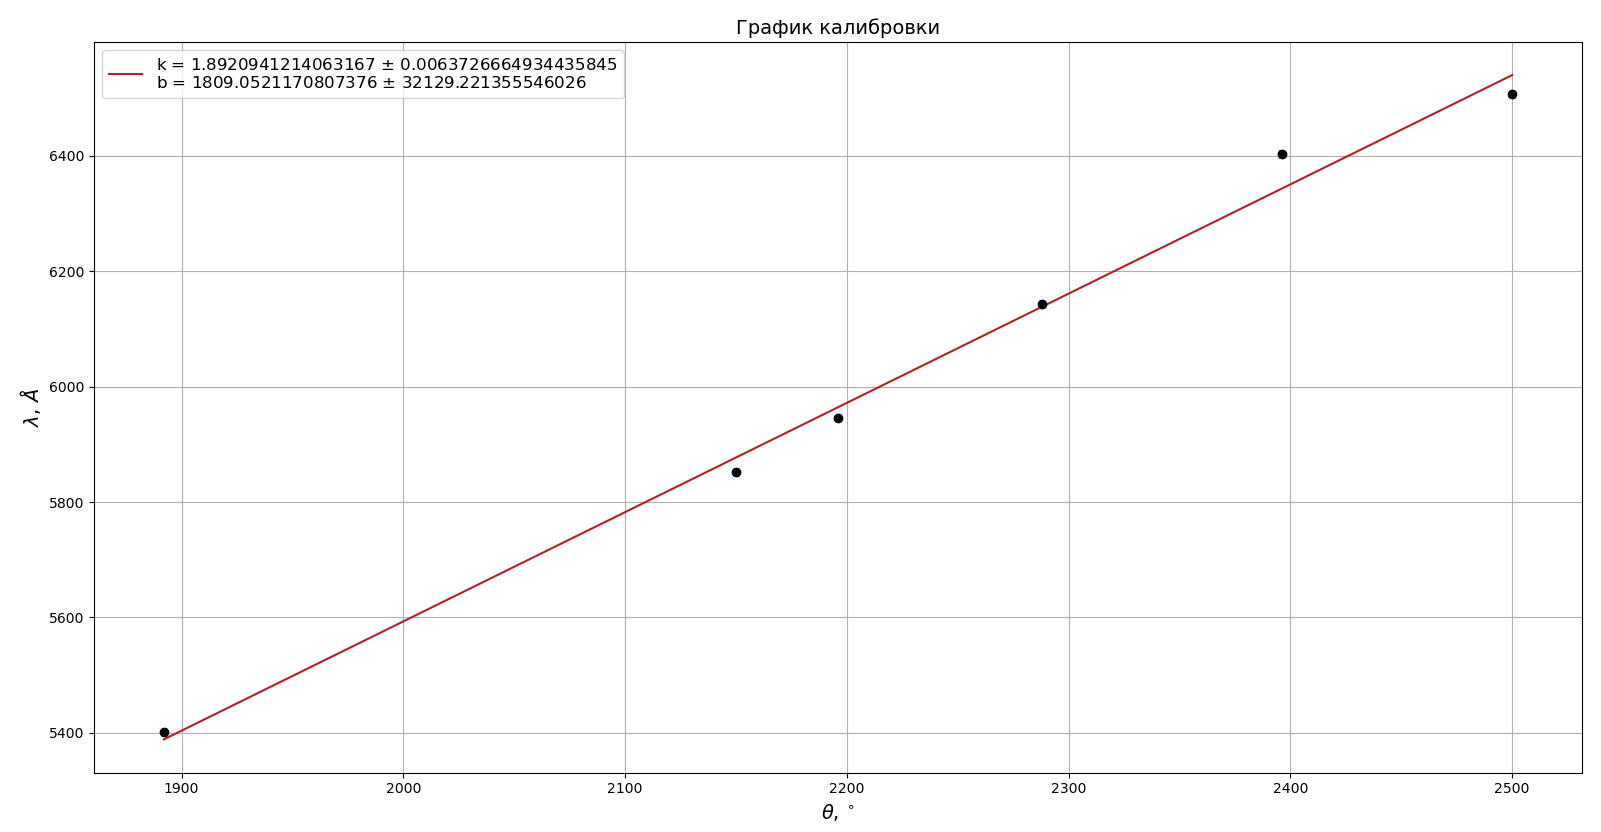
\includegraphics[width = \textwidth]{colibrovka.png}
		\caption{Калибровка} 
	\end{figure}

	Теперь проведем 5 серий измерений зависимости фототока от напряжения для разных длин волн падающего света, изменяя на монохроматоре параметр $ \theta $ и переводя его в длину волны с помощью градуировки. Ток приведен в безразмерных единицах в силу работы установки. 
	
	\begin{table}[h]
		\centering
		\caption{$U_I$ для соответствующих $\lambda$ и  $U$}
		\begin{tabular}{|c||c|c|c|c|c|c|} \hline
			 			& $\lambda = 1690$\AA & $\lambda = 1790$\AA & $\lambda = 1890$\AA & $\lambda = 1990$\AA & $\lambda = 2090$\AA \\ \hline \hline
			$U = -0.6$  & 0.021 & 0.016 & 0.000 & 0.011 & 0.007 \\ \hline
			$U = -0.55$ & 0.039 & 0.031 & 0.010 & 0.027 & 0.01  \\ \hline
			$U = -0.5$  & 0.059 & 0.052 & 0.032 & 0.050 & 0.029 \\ \hline
			$U = -0.45$ & 0.081 & 0.075 & 0.059 & 0.078 & 0.056 \\ \hline
			$U = -0.4$  & 0.107 & 0.103 & 0.090 & 0.112 & 0.088 \\ \hline
			$U = -0.35$ & 0.133 & 0.134 & 0.129 & 0.148 & 0.122 \\ \hline
			$U = -0.3$  & 0.166 & 0.168 & 0.172 & 0.191 & 0.165 \\ \hline
			$U = -0.25$ & 0.199 & 0.205 & 0.218 & 0.236 & 0.212 \\ \hline
			$U = -0.2$  & 0.230 & 0.242 & 0.264 & 0.279 & 0.263 \\ \hline
		\end{tabular}
	\end{table}

	\begin{figure}[H]
		\centering
		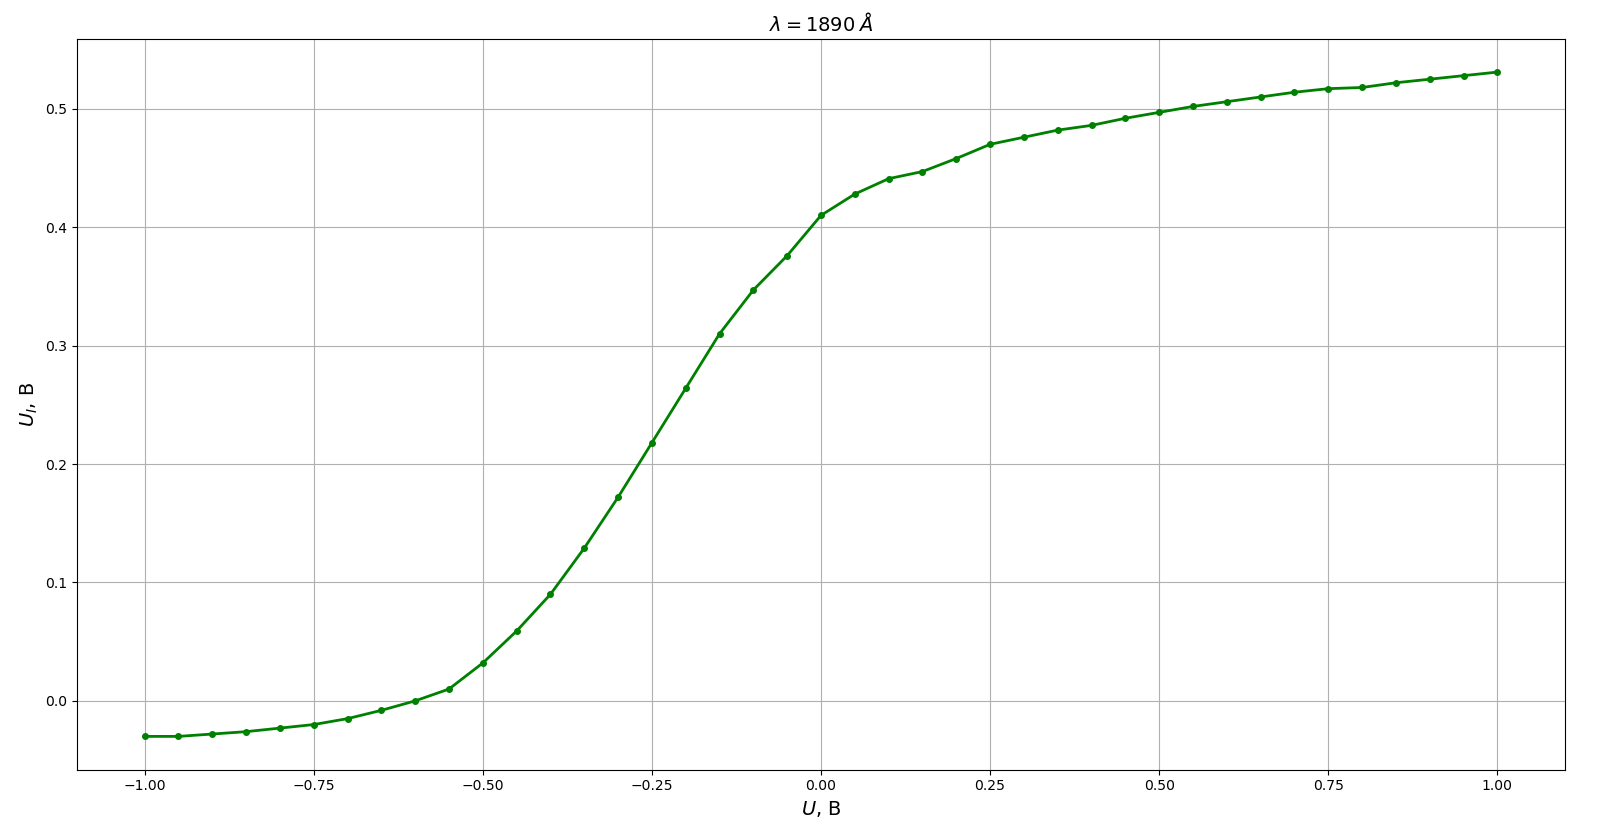
\includegraphics[width = \textwidth]{photoeffect.png}
		\caption{Зависимость фототока от напряжения для $\lambda = 1890$ \AA} 
	\end{figure}

	\begin{figure}[H]
		\centering
		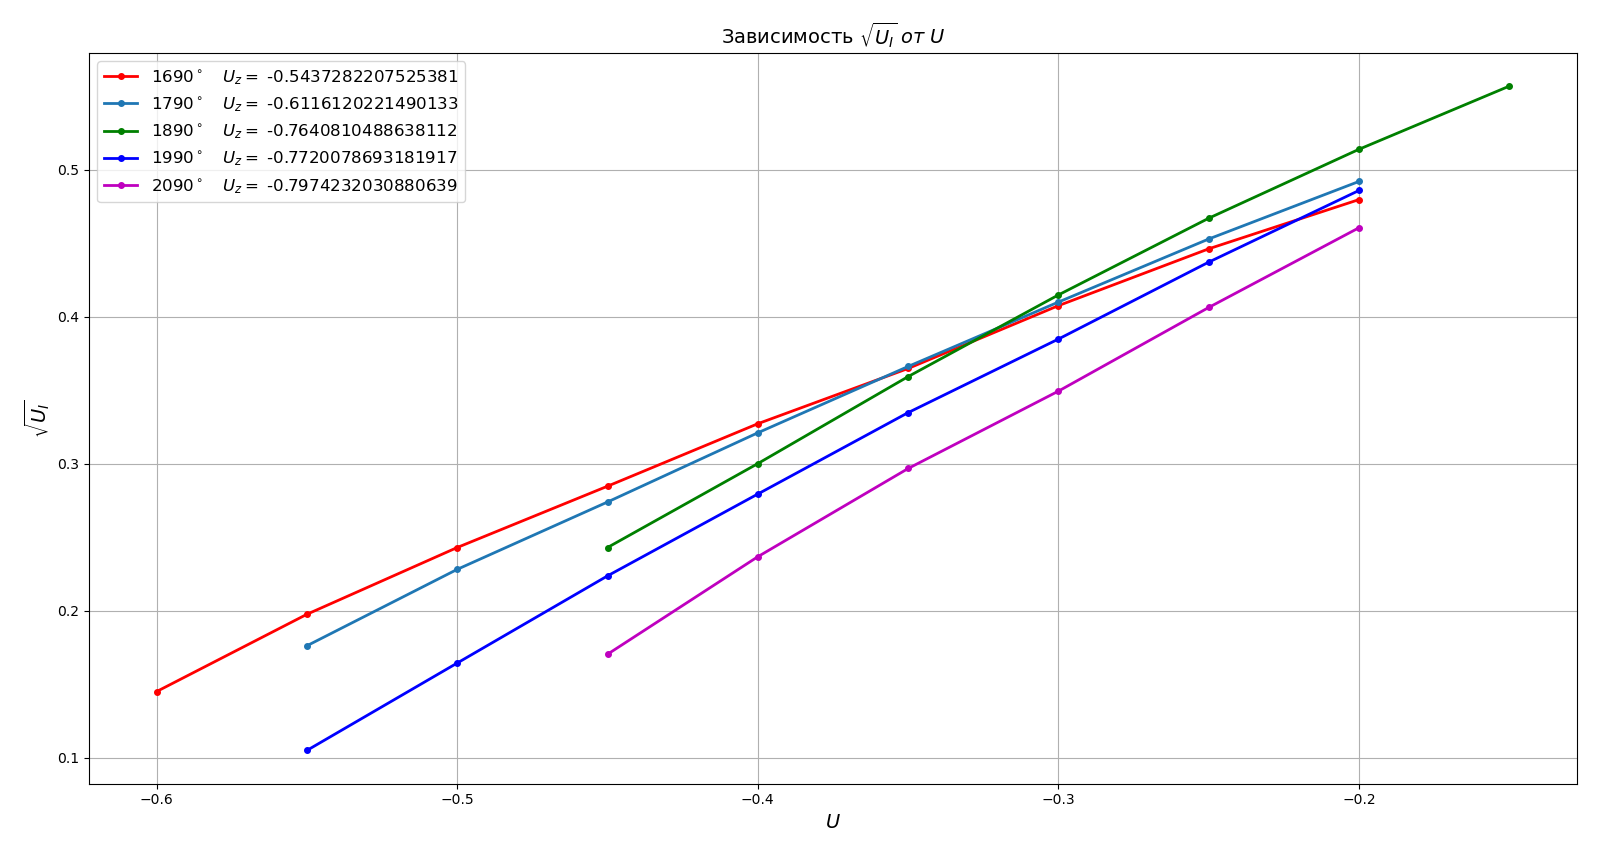
\includegraphics[width = \textwidth]{all.png}
		\caption{Корень из зависимости фототока от напряжения} 
	\end{figure}

	Вблизи потенциала запирания, искомая зависимость описывается формулой \eqref{sqrt I = V}. 
	Согласно этой формуле \eqref{sqrt I = V}, построим график зависимости в координатах 
	$ \sqrt{I} (V) $ и аппроксимируем линейные участки прямой. Экстраполируя прямую к нулю, 
	получим значения потенциала запирания для каждой серии измерения (длины волны). 

	\begin{table}[h]
		\centering
		\caption{$U_{\text{зап}}$ для соответствующих $\lambda$}
		\begin{tabular}{|c||c|c|c|c|c|c|} \hline
			$\lambda$, \AA & 1690 & 1790 & 1890 & 1990 & 2090 \\ \hline
			$U_z$ & -0.544 & -0.612 & -0.764 & -0.772  & -0.797 \\ \hline		
		\end{tabular}
	\end{table}

	\begin{figure}[H]
		\centering
		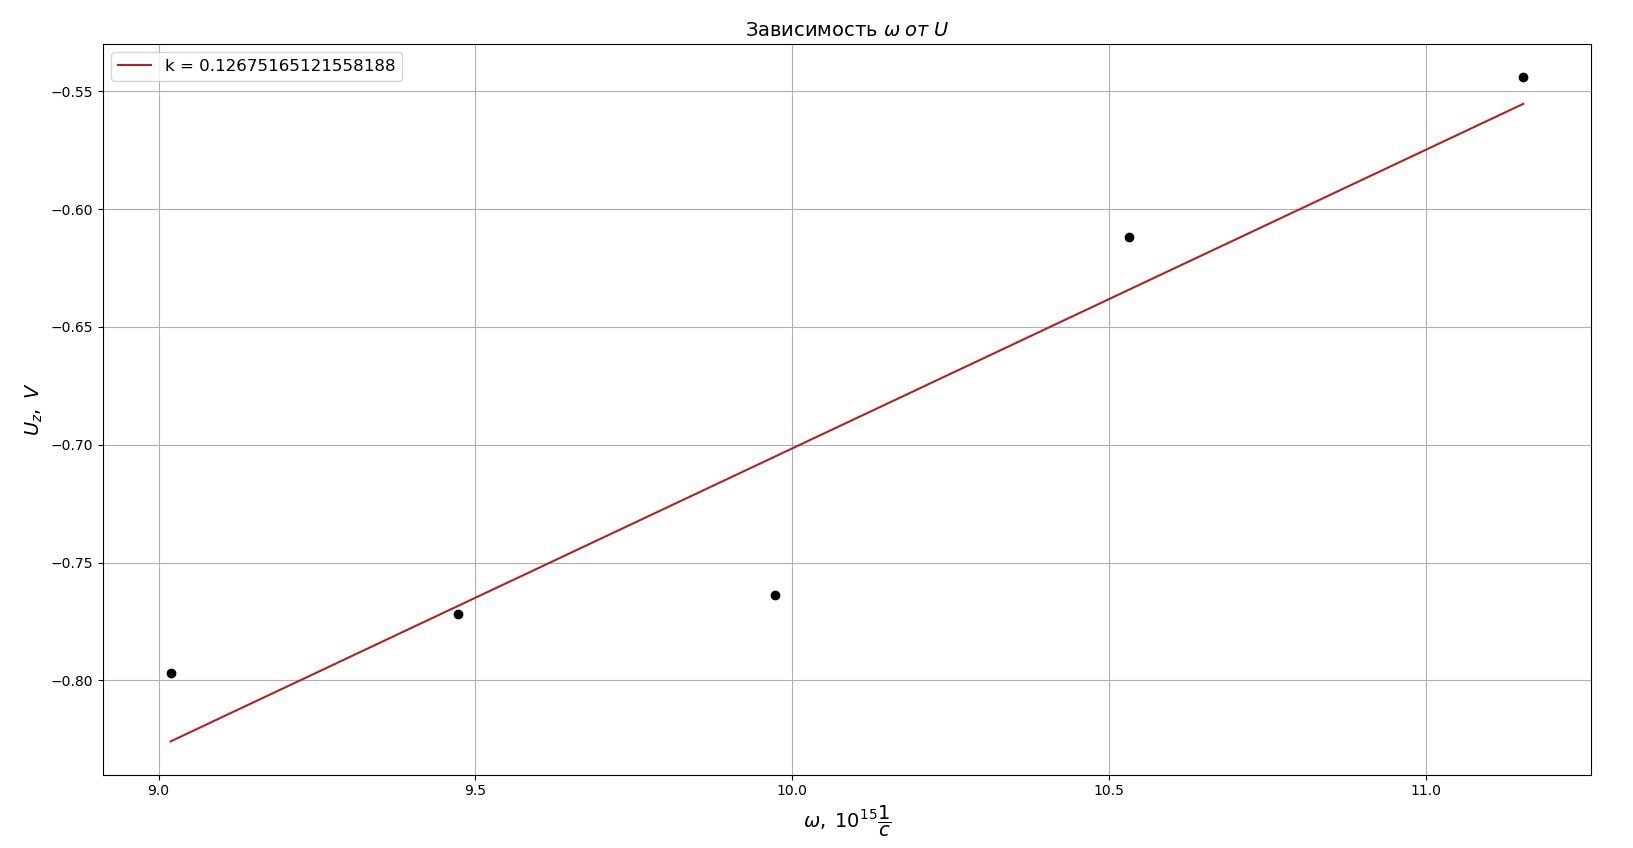
\includegraphics[width = \textwidth]{ashnu.png}
		\caption{Зависимость запирающего потенциала от циклической частоты} 
	\end{figure}

	\begin{equation*}
		\frac{\hbar}{e} = k = (0.126 \pm 0.005) \cdot 10^{-15} \; \dfrac{\text{Дж}\cdot\text{с}}{\text{Кл}}
	\end{equation*}
	\begin{equation*}
		\hbar = 0.2 \cdot 10^{-34} \; \text{Дж}\cdot\text{с}
	\end{equation*}
        	 
	По порядку это согласуется с табличным значением $ \hbar = 1,054 \cdot 10^{-34} \; \text{Дж} \cdot \text{с} $.

	\section{Вывод}
	
	Таким образом, в ходе выполнения работы мы проверили Энштейновское описание фотоэффекта и с помощью уравнения последнего измерили постоянную Планка. Результат по порядку соответствуют табличному значению.
	


\end{document}